\documentclass[reprint,amsmath,amssymb,aps,12pt]{article}

\usepackage{graphicx,dcolumn,bm,mathrsfs,subfigure,tikz,pgf,times}
\usetikzlibrary{shapes,arrows}

\begin{document}

\begin{figure}
	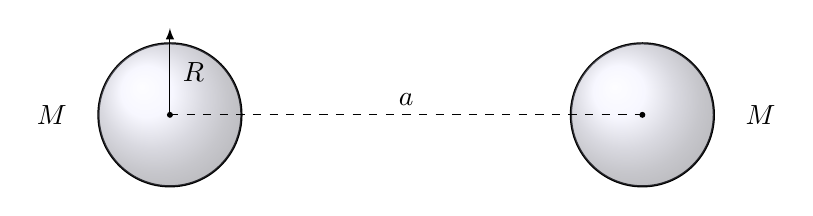
\begin{tikzpicture}[>=latex,scale=2]
		% Draw binary and associated geometry.
		\draw[black,fill=white,thick] (2,0) circle (3ex);
		\shade[ball color=blue!10!white,opacity=0.40] (2,0) circle (3ex);
		\draw[black,fill=white,thick] (-1,0) circle (3ex);
		\shade[ball color=blue!10!white,opacity=0.40] (-1,0) circle (3ex);
		\draw[dashed] (-1,0) -- (2,0);
		\draw[black,fill=black] (-1,0) circle (.1ex);
		\draw[black,fill=black] (2,0) circle (.1ex);

		% Draw binary labels.
		\draw[->] (-1,0) -- (-1,0.55);
		\draw (-0.85,0.15) node[above]{$R$};
		\draw (0.5,0) node[above]{$a$};
		\draw (2.75,0) node{$M$};
		\draw (-1.75,0) node{$M$};
	\end{tikzpicture}
\end{figure}

\end{document}
